\section*{Interfaz entre medios}

\item 
\begin{enumerate}
	\item (*) Demuestre que la función: $\Psi (\vec{r}, t) = A \operatorname{e}^{ i (\vec{k} \cdot \vec{r} \pm \omega t) }$, con $\vec{k} = k_x \hat{x} + k_y \hat{y} + k_z \hat{z}$ un vector constante y $\vec{r}= x \hat{x} + y \hat{y} + z \hat{z}$, es solución de la ecuación de ondas tridimensional.
	Sugerencia: exprese el Laplaciano en coordenadas cartesianas.
	\item Analice el significado físico de $\Psi (\vec{r}, t)$.
	¿Cómo son los frentes de onda?
	¿Cuál es la relación entre el vector $\vec{k}$ y los frentes de onda?
	¿Hacia dónde se desplazan los frentes de onda al transcurrir $t$?
	¿A qué velocidad?
\end{enumerate}


\item (*)
\begin{minipage}[t][2cm]{0.75\textwidth}
Una onda de presión \( \delta p_i (\vec{r},t)\) incide desde el aire describiendo un ángulo $\theta$ con la normal a una superficie de agua calma.
Si usamos notación compleja la describimos como $\delta p_{i} (\vec{r}, t) = A_i \operatorname{e}^{i (\vec{k}_{i} \cdot \vec{r} - \omega t) }$, siendo $\vec{k}_i = \frac{ \omega }{ v_s } \left( \sen(\theta) \hat{x} + \cos(\theta) \hat{y} \right)$.
Hallar las ondas reflejadas y transmitidas, $\delta p_r (\vec{r}, t) = A_r \operatorname{e}^{ i ( \vec{k}_r \cdot \vec{r} - \omega t) }$ y $\delta p_t (\vec{r}, t) = A_t \operatorname{e}^{ i (\vec{k}_t \cdot \vec{r} - \omega t) }$.
\end{minipage}
\begin{minipage}[c][0.4cm][t]{0.2\textwidth}
	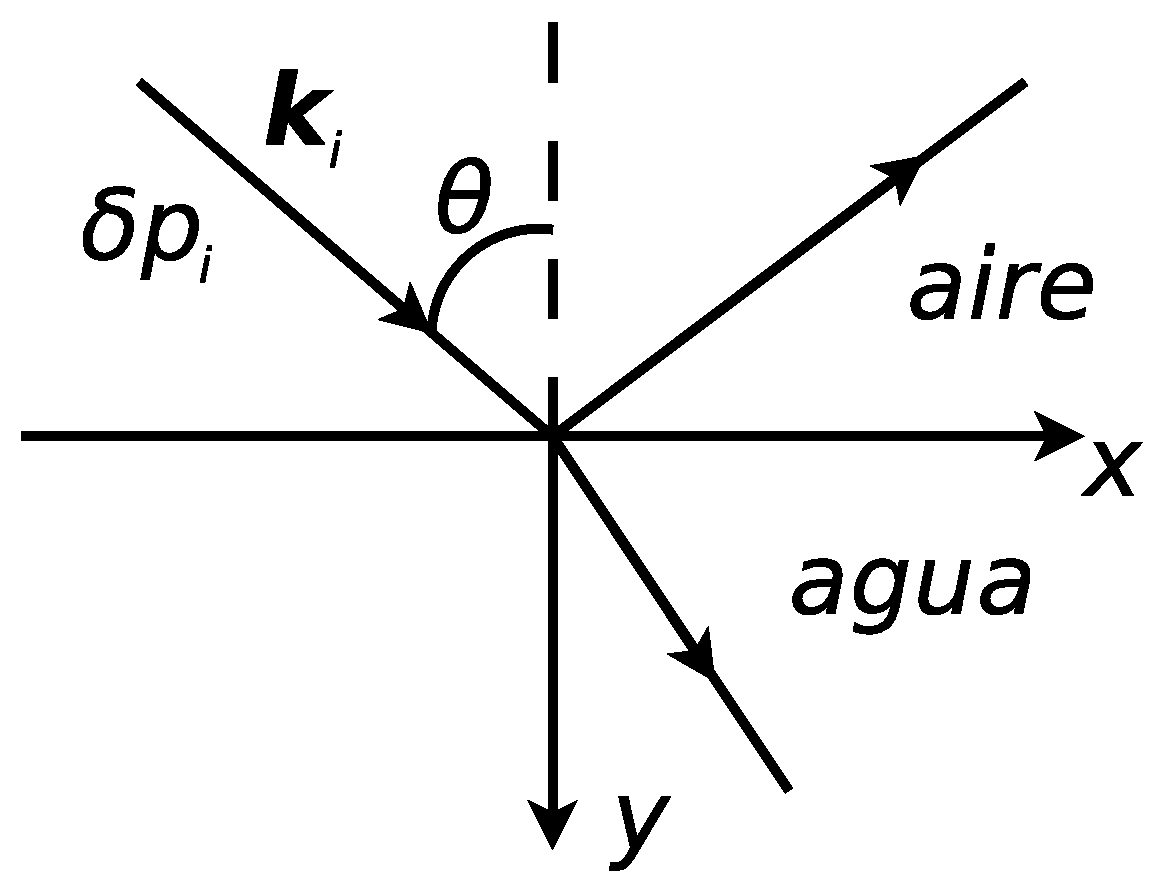
\includegraphics[width=\textwidth]{ej2-13}
\end{minipage}
